\documentclass[prl,twocolumn]{revtex4-1}

\usepackage{graphicx}
\usepackage{color}
\usepackage{latexsym,amsmath}

\definecolor{linkcolor}{rgb}{0,0,0.65} %hyperlink
\usepackage[pdftex,colorlinks=true, pdfstartview=FitV, linkcolor= linkcolor, citecolor= linkcolor, urlcolor= linkcolor, hyperindex=true,hyperfigures=true]{hyperref} %hyperlink%


\begin{document}

\title{2216 -- Some catch title for the assignment}

\author{Ema Baci}
\author{Christoffer Askvik Faugstad}
\author{Melika Keshavarzmirzamohammadi}
\author{Veslemøy Therese Svendby Osmundsen}

\date{\today}

\begin{abstract}
An investigation was done to determine how different hyper parameters in a deep neural network impacts its performance. The architecture of the network, training parameters and initialization of the layers in the model was tuned by using grid search, yielding the best possible model for the task. It was found that a smaller sample size for training is sufficient to yield a good accuracy as long as the number of epochs is increased, and that in the case of limited data points, augmentation serves well as an artificial generator of more samples. For the simple task of binary classification of points, several combinations of parameters yielded good results which indicated that a very complex network was ambiguous for our classification task. 

\end{abstract}

\maketitle

\section{Introduction}
In this task a sequential deep neural network was built to perform binary classification of points. The aim was to predict whether a given point in a grid of size $\left[-50,50\right]$ was classified within the boundaries of a chosen shape or pattern. In our experiments a triangle was used as the geometrical shape, and hence the final network model was tuned for that purpose. The network parameters chosen may also work well for training of other simple shapes, but for more complex patterns, a more complex model is needed. Nevertheless, the triangle works well to show the impact of the different parameters on the network.

%%%%%%%%%%%%%%%%%%%
%\begin{figure*}[!tb]
%  \centering
%%  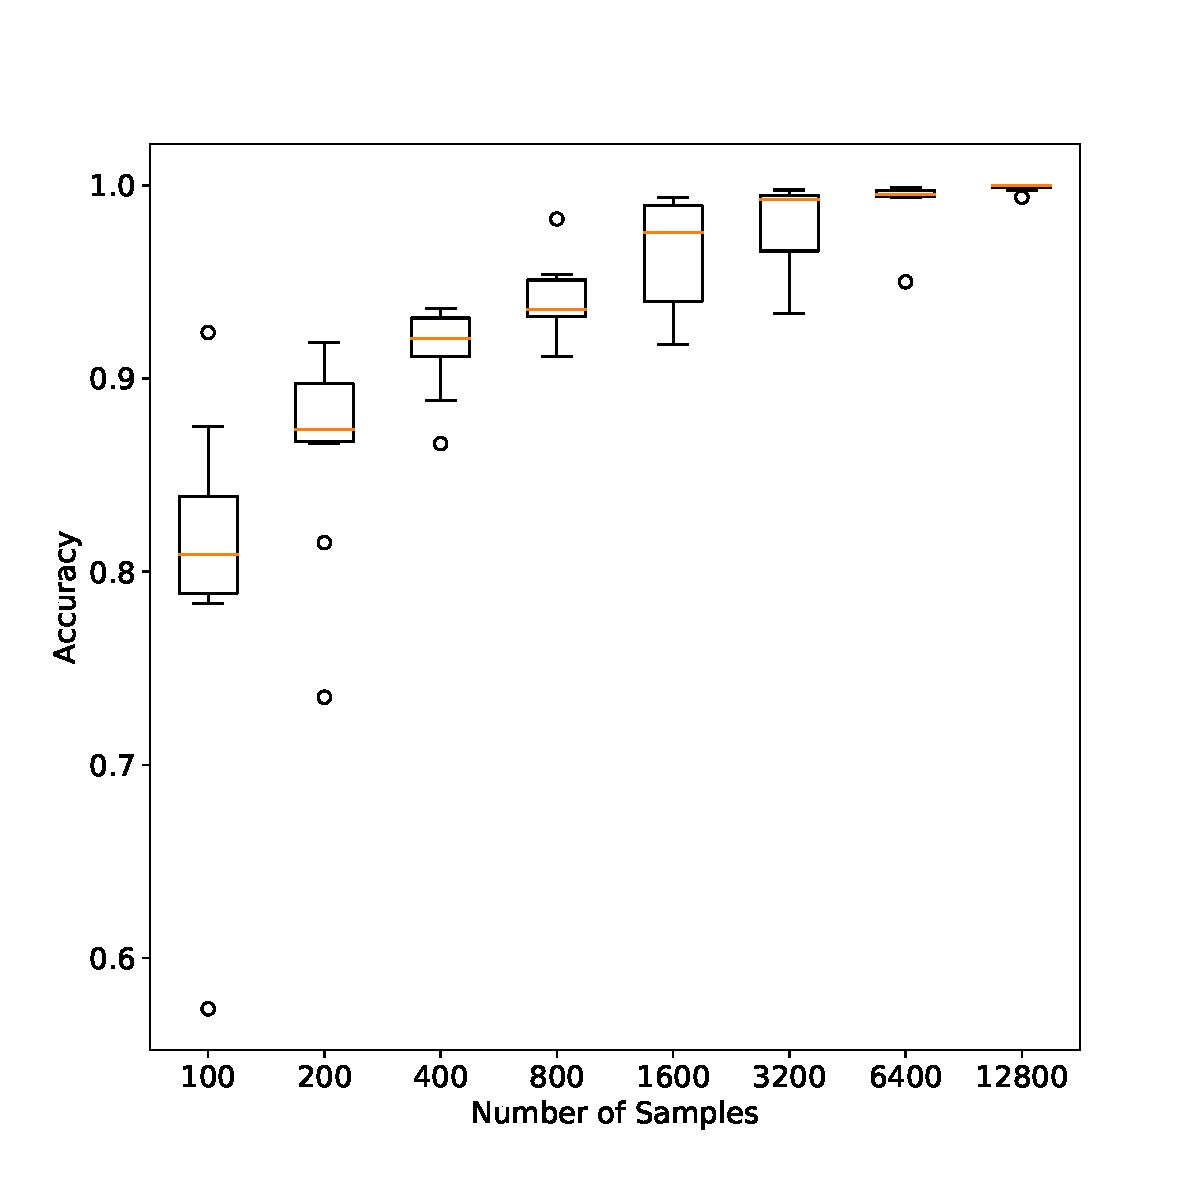
\includegraphics[width=0.3\textwidth]{task_1/num_train_box.pdf}
%  \caption{Description of the panels: (a)..... (b)... etc. This %caption should give enough info on the content of figures to %make them mostly readable without consulting the main text. %However, repetitions with the main text should e avoided if %possible. {\color{red} If this format is difficult to frame in %the page you want, just break it into multiple single %figures.}}
%  \label{fig:x}
%\end{figure*}
%%%%%%%%%%%%%%%%%%%

 \section{Methods}
In this section the methods used to characterized a Neural Network (NN) built with Keras library are discussed. First of all the NN was trained with several training sets with different sizes, then the response of the NN to augmented training sets was studied. 
After that it was possible to understand which was the best training set size that optimizes both the accuracy and the computational time. The performance of the NN was then further improved through a Grid Search Validation process, that leads to the best parameters and though the optimization of the initial weights.
%\subsection{Problem} % Not to be kept
%A binary classification problem in two dimensions is considered where the samples are labeled by a non-linear function. The samples have each component drawn uniformly and uncorrelated from the range $[-50,50]$. The main non-linear function used is the triangle, described by the function 
%\begin{equation}
%f(x_1,x_2) = \begin{cases} 1,\
%x_1\in [-20,80] \wedge x_2 \in [-40,80-x_1]\\
%0, \ \textrm{else}.
%\end{cases}
%\end{equation}
%Other functions used for labeling are shown in figure
% \ref{fig:domains}. % Not sure if this should be present.
%They are used to see how the found network performs on a more complex function. 
%\\
\subsection{General model}
The network model was created by using Keras.Sequential(), which yields a fully connected deep neural network. The hidden layers are of the type Dense, with the activation function and number of nodes as inputs. Each Dense layer is alternated to a dropout one with rate , and the sigmoid function is given as activation in the final layer. The different parameters of the architecture of the network was given by input to the model compiler in order to apply grid search for tuning. Hence, the final architecture of the network was determined by the findings of our research.

\subsection{Initialization and activation functions}
The activation functions tested in our model were sigmoid, relu(rectified linear unit), and elu(exponential linear unit), given respectively as
\begin{equation}
    \sigma(x) = \frac{1}{1+e^{-x}},
    \label{eq:sigmoid}
\end{equation}
\begin{equation}
    f_\textrm{relu}(x) = \max \{0,x\}
    \label{eq:relu}
\end{equation}

\begin{center}
and
\end{center}
\begin{equation}
    f_\textrm{elu}(x) = \begin{cases}.
    x, \ \ \ \ \ \ \ \, x \geq 0\\
    e^x -1, \ x < 0
    \end{cases}
    \label{eq:elu}
\end{equation}

% The training of a neural network is also very sensitive to its initial weights.
In keras the default initialization of the initial weights is a glorot uniform distribution. The glorot uniform distribution is specially designed for the sigmoid activation function, and draws values uniformly from the interval $-[\textrm{limit},\textrm{limit}]$. The limit is given by 
\begin{equation}
    \textrm{lim}_\textrm{Glorot} = \sqrt{\frac{6}{\textrm{fan}_{in}+\textrm{fan}_{out}}},
\end{equation}

where $\textrm{fan}_{in}$ and $\textrm{fan}_{out}$ denotes the number of input and output layers respectively. However, the glorot initialization is not necessarily the best option for the rectified linear unit activation function. The limits of the He uniform distribution is given as
\begin{equation}
    \textrm{lim}_\textrm{He} = \sqrt{\frac{6}{\textrm{fan}_{in}}},
\end{equation}
depending only on the number of input layers. This is normally a better option for the rectified linear unit activation function. Both distributions were tested to initialize the weights of our model.
\\
When re-scaling the data three methods are considered. Since the actual distribution is known the first is to divide by $50$ giving a uniform distribution between $[-1,1]$. The equivalent of this when the sample distribution is unknown is to normalize the data by using the max and min of the training samples. The third approach considered it to standardize. Then the mean is subtracted and its divided by the standar diviation of the training samples.  



\subsection{Handling Uncertainty}
The training process of the network is a stochastic process and therefore the obtained accuracies greatly depend on the initial weights. Because of this each network is trained from 30 fixed initial weights (only if the architecture is identical) and the results are displayed as box-plot to illustrate the variance. If a gird search is done there is instead used 5 fold cross validation.

\subsubsection{Number of training samples}
The effect of the achieved accuracy of the neural network given the number of samples was found by fixing the architecture and the training procedure and only changing the number of training samples in use. In particular the neural network was trained with eight different training sets, with sizes from 100 to 12800, all generated by the same distribution.


\subsubsection{Augmenting data}
% With limited data samples, augmentation can be used to artificially generate more data.
The data points were artificially augmented by adding a small perturbation to each of the components of the original samples. The small perturbations are drawn uniformly from $[-0.05,0.05]$. To investigate the impact of the augmentation, different ratios of augmented to original samples in the training set were tested, while holding the number of original training samples fixed.\\


\subsection{Gridsearch}
There are many parameters to be determined in a neural network. Grid search is an effective way of finding the optimal combination of hyper parameters and was the method used for the finetuning of our model. The parameters were divided into the three categories; arcitecture, training and initialization, and a grid search was done for each category.

To determine the architecture of the network, a grid with varying number of nodes, number of layers, dropout rate, hidden layers and activation function was done, using cross validation.

To determine the training parameters, a grid with varying batch size, optimizer and number of epochs was done while having a fixed architecture of the network, and using the default initialization function in keras and cross validation.

To find the best initialization conditions, a grid with varying initialization function and activation function was done with cross validation, while the architecture and training parameters were held fixed.




\begin{table}[!b]
\begin{center}
\begin{tabular}{ll}
quantity & value \\
\hline
initialization function of weights & He uniform\\ 
initial activation function & relu \\
hidden layers activation function & relu\\
final activation function & Sigmoid \\
number of hidden layers & $4$ \\
number of nodes hidden layers & $10$\\
dropout & $0.0$\\
optimizer & adam\\
epochs & $200$ \\
batch size & 16\\
training samples & 3200\\
validation samples & 800\\
target function & triangle
\end{tabular}
\end{center}
\caption{The default parameters used for the network architecture and its training parameters.}
\label{tab:optimal_value}
\end{table}


\section{Results}
\begin{table}[!b]
\begin{center}
\begin{tabular}{llllll}
\hline
accuracy(std) & time[s] & layers & nodes & dropout & afunc \\
\hline
0.977 (0.029) & 9.77 & 3 & 40 & 0.0 & relu\\
0.980 (0.026) & 9.84 & 4 & 10 & 0.0 & relu\\
0.988 (0.020) & 10.74 & 4 & 40 & 0.0& relu\\
\hline
\end{tabular}
\end{center}
\caption{The best architectures found from grid search with cross validation with 5 folds. Time is the average time used to train the network. Layers is the number of hidden layers, searched over the values 2,3,4. Nodes are the number of nodes in each hidden layer, the values used for the grid were 10,20,40. Dropout is the dropout rate of the nodes in the hidden layers. The values 0 and 0.1 were checked. Afunc is the activation function used in the hidden layers, where sigmoid, relu and elu were the alternatives. The presented accuracy is the average value when the model is trained from 10 different initial weights.}
\label{tab:grid_search_architecture}
\end{table}


\begin{table}[!b]
\begin{center}
\begin{tabular}{lllll}
\hline
accuracy(std) & batch size & epochs & optimizer \\
\hline
0.964 (0.034) & 16 & 400 & Adam\\
0.950 (0.030) & 4 & 400 & RMSpropu\\
0.961 (0.029) & 4 & 40 & 0.0& relu\\
\hline
\end{tabular}
\end{center}
\caption{The best training parameters found from grid search with cross validation with 5 folds. The presented accuracy is the average value when the model is trained from 10 different initial weights. The batch size is the number of samples used for each update. The epochs are the number of times the training set has been looped through. The optimizer is the optimizing algorithm used to train the network. The default architecture is used.}
\label{tab:grid_search_training}
\end{table}

\subsection{Variations in the training set}

From figure \ref{fig:num_train_samples} there is a clear correlation between number of training samples and the average accuracy. The increased accuracy approach the optimal value. There is also a smaller spread in the obtained accuracies as the number of training samples increases. From the data one can conclude that $3200$ training is a satisfactory compromise between accuracy and computation time. The larger values of training samples has the same similar average, but considerably less variation. 


\subsection{Augmented data}
The accuracies obtain over 10 runs, each with different proportions of augmented data compared to real data. \ref{fig:augmented_train_sampels}. The figure shows that adding extra augmented samples decrease the average accuracy, but at the expense of this the spread of the data is smaller.


\begin{figure}[ht]
  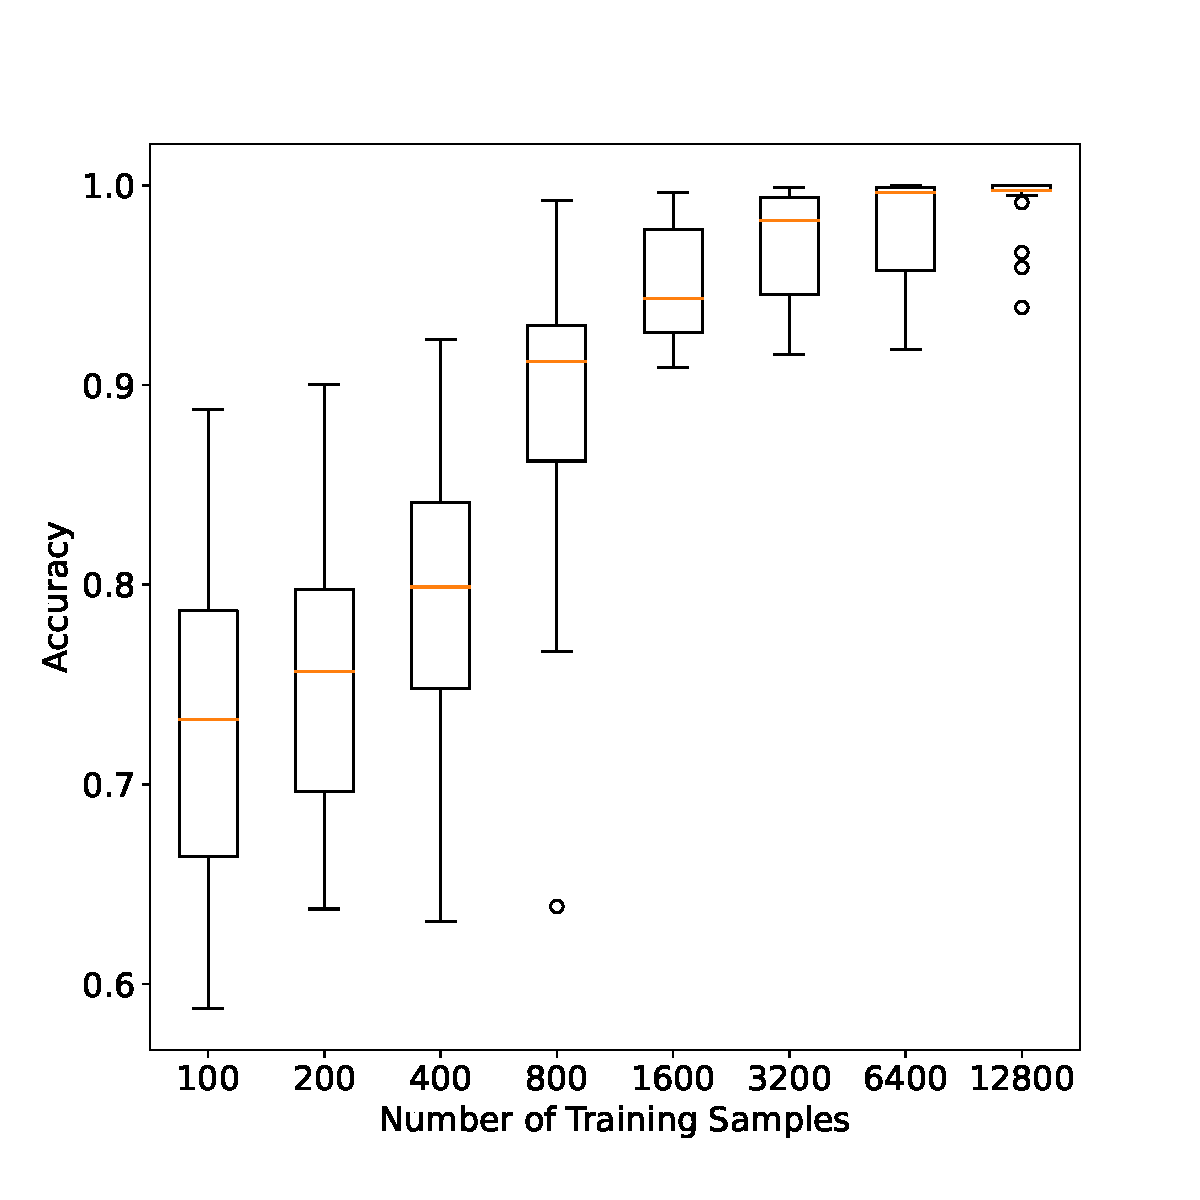
\includegraphics[width=0.44\textwidth]{task_1/num_train_box_30.pdf}
  \caption{The accuracy's achieved by the default network with a varying number of training samples. Each started from 10 different initial weights.}
  \label{fig:num_train_samples}
\end{figure}


\begin{figure}[!tb]
  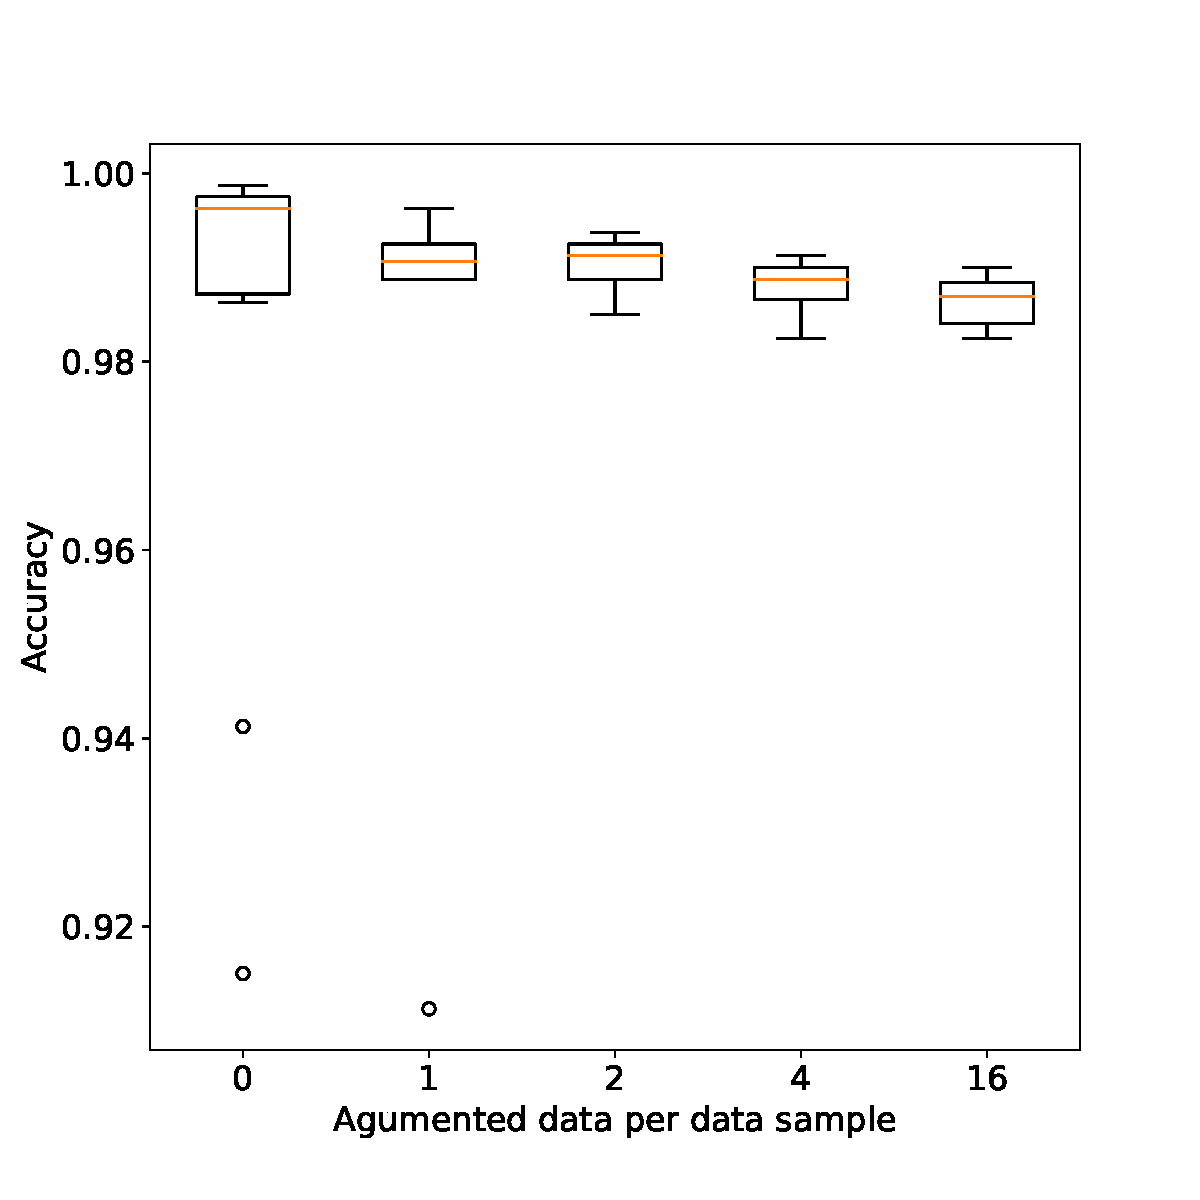
\includegraphics[width=0.44\textwidth]{ag_train_box.pdf}
  \caption{The different accuracies achieved by the default network when adding the indicated number of augmented data per original training data. The values are for 10 different initial weights for each augmented data per original training data. The original training data consist of $3200$ samples.}
  \label{fig:augmented_train_sampels}
\end{figure}


\begin{figure}[!tb]
  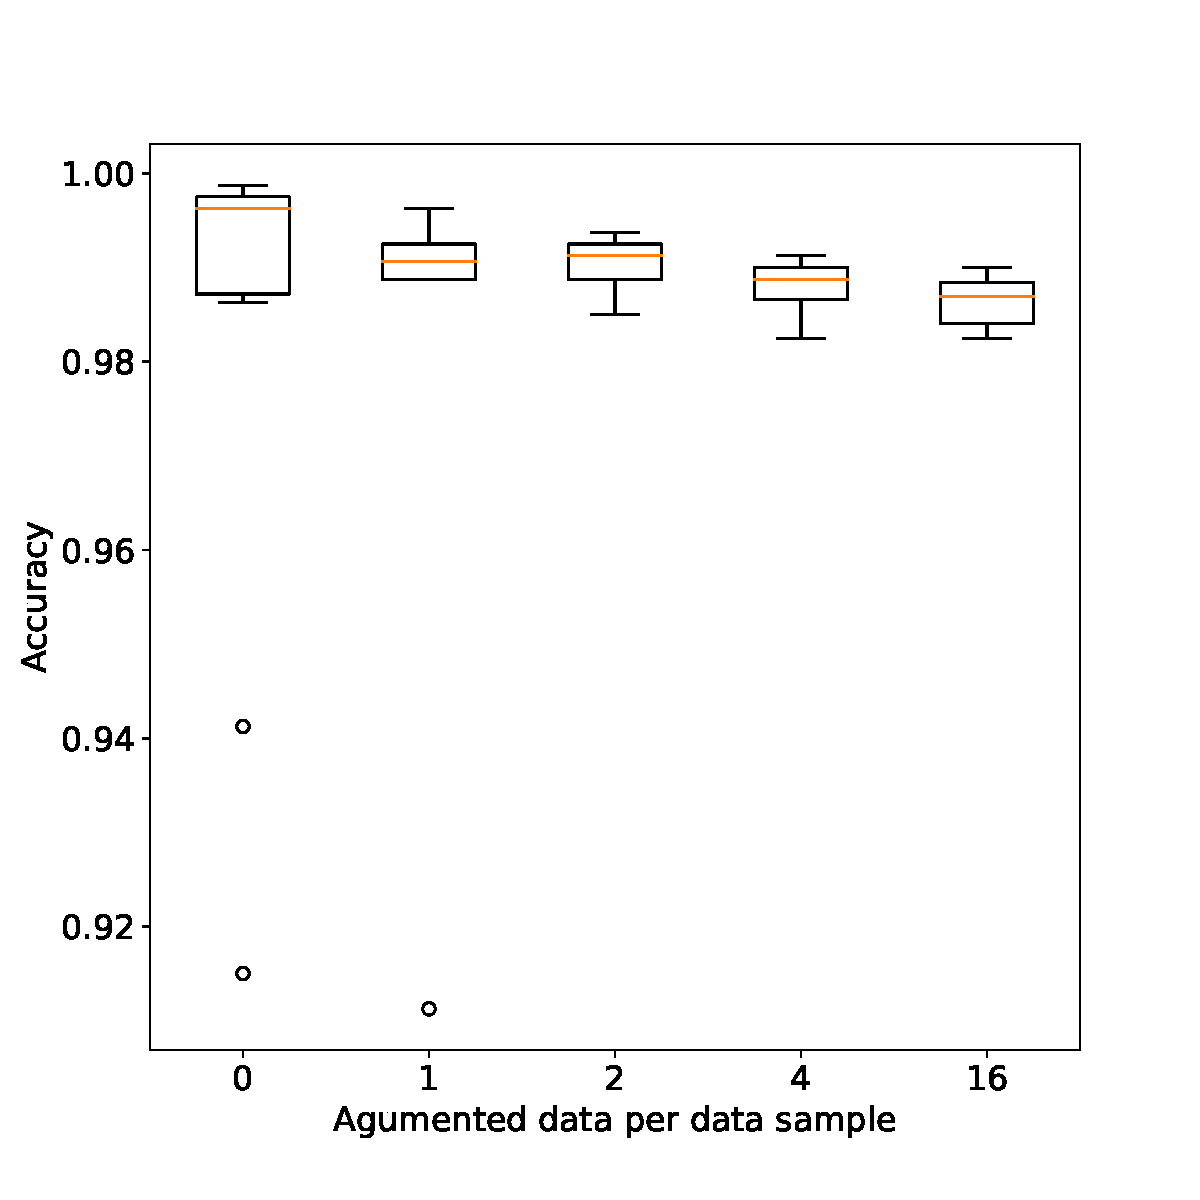
\includegraphics[width=0.44\textwidth]{
  ag_train_box.pdf % Need to be changed
  }
  \caption{
  The distribution of accuracies achieved with different initialization distributions. 
  }
  \label{fig:weight_init_box}
\end{figure}


\begin{figure}[!tb]
  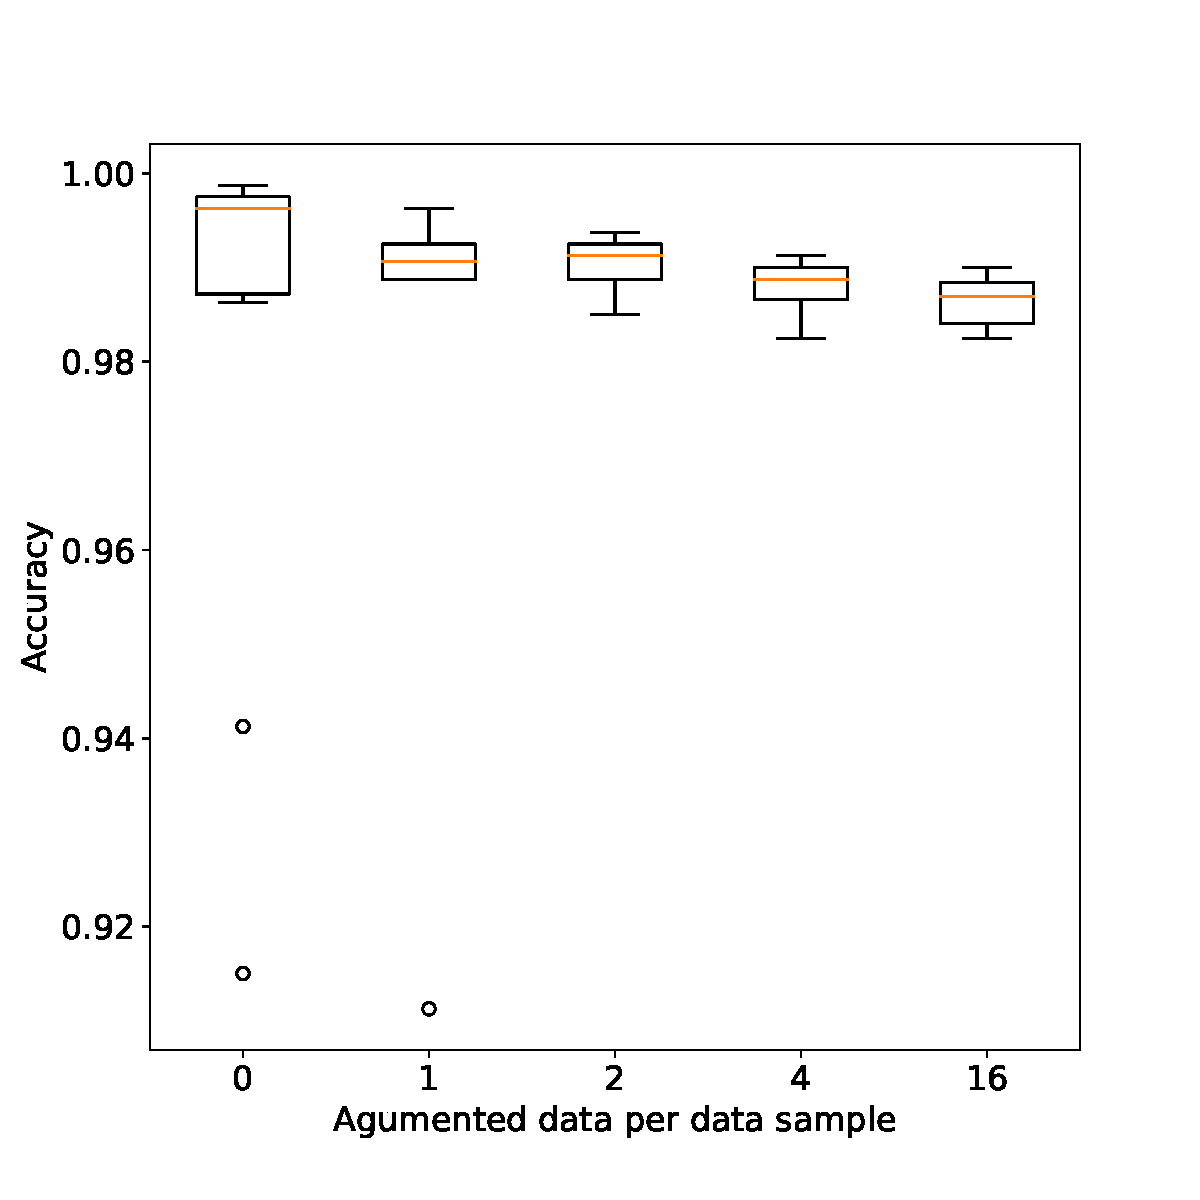
\includegraphics[width=0.44\textwidth]{
  ag_train_box.pdf % Need to be changed
  }
  \caption{
  The distribution of accuracies achieved with different re-scaling methods. 
  }
  \label{fig:rescale_box}
\end{figure}

\begin{figure}[!tb]
  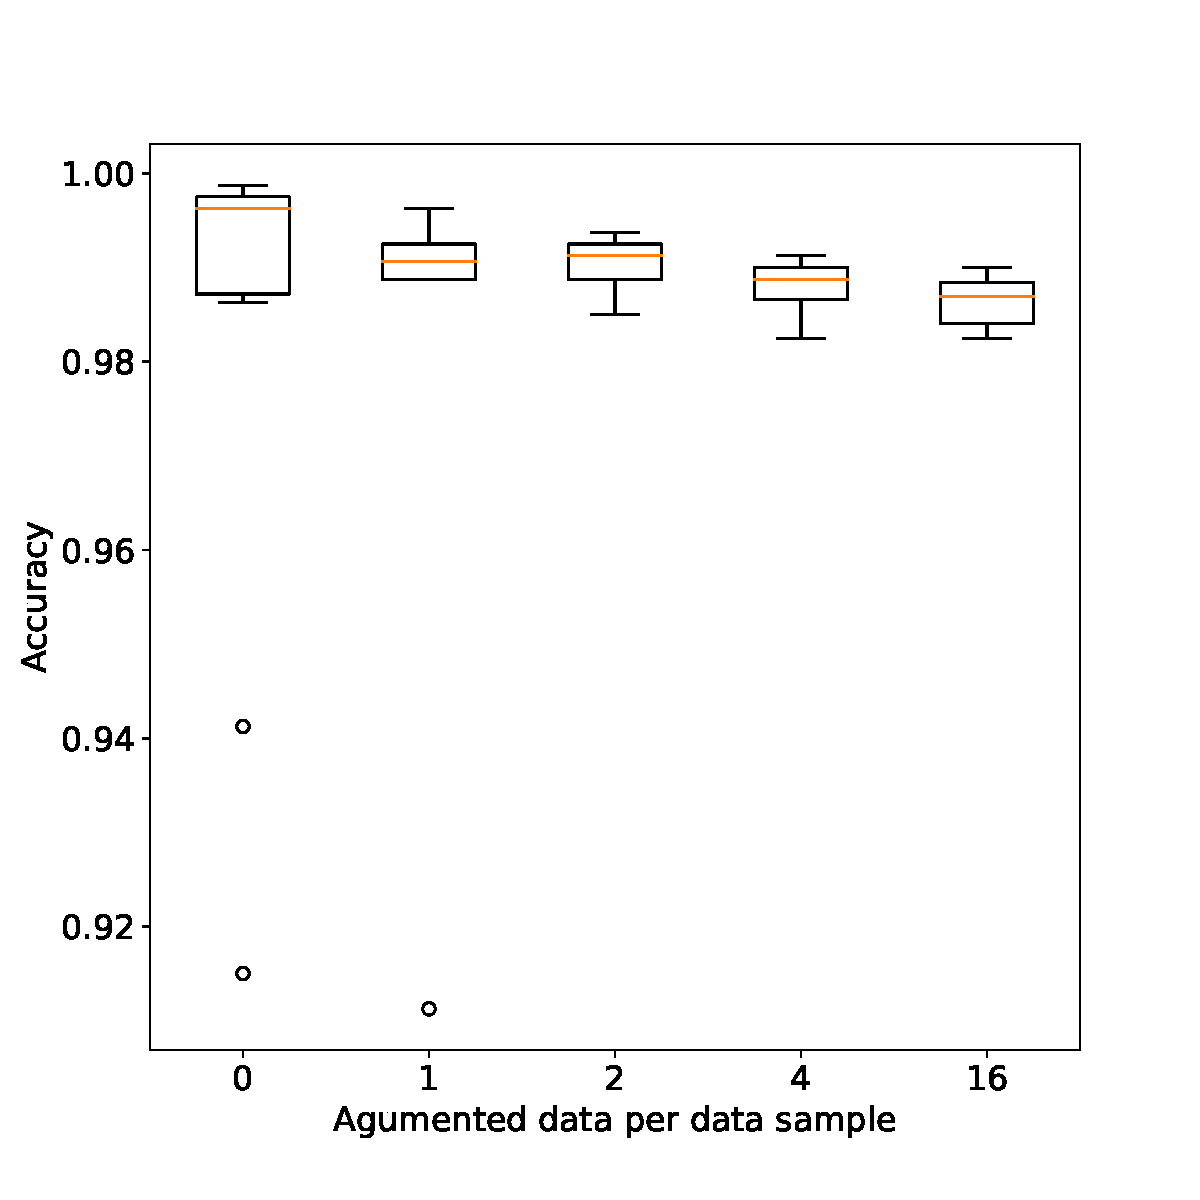
\includegraphics[width=0.44\textwidth]{
  ag_train_box.pdf % Need to be changed
  }
  \caption{
  The distribution of accuracies for the different non-linear functions used to label the points. 
  }
  \label{fig:rescale_box}
\end{figure}




\section{Conclusions}


Check if your text is light, swift, and correct in exposing its passages.





\begin{thebibliography}{99}

\bibitem{pap1}
  B. Franklin,
  J. Here There {\bf 10}, 20--40 (1800).
  
\bibitem{pap2}
  A. Einstein,
  Int. J. There Here {\bf 20}, 125--133 (1910).
  
\end{thebibliography}

\clearpage

% %%%%%%%%%%%%%%%%%%%
% \begin{figure*}[!tb]
%   \centering
%   \includegraphics[width=\textwidth]{description_assignment_LCPB_20-21.pdf}
% \end{figure*}
% %%%%%%%%%%%%%%%%%%%


\end{document}
















% Templates that might be needed


\begin{table}[!b]
\begin{center}
\begin{tabular}{lll}
quantity & symbol & dimensionless \\
\hline
time & $t$ & $t'$  \\
momentum & $p$ & $v$
\end{tabular}
\end{center}
\caption{Description of the table.}
\label{tab:1}
\end{table}









\subsection{Classification}
The rectangle for labeling the samples was given by the limits
\begin{equation}
f(x_1,x_2) = \begin{cases} 1,\
x_1\in [-20,80] \wedge x_2 \in [-40,80-x_1]\\
0, \ \textrm{else}
\end{cases}
\end{equation}





